%****************************************************************
% Chapter X
%****************************************************************
\label{ChapterX}
\chapter{Chapter To Be Removed}

%****************************************************************
\section{Ray Intersection}

Detect collisions between ray and models is the key to allow user selecting objects in the VR would, which is one of the importent experience for user interaction.

A ray can be describe in a equation with known ray start position \emph{$\overrightarrow{R_{0}}$} and ray direction \emph{$\overrightarrow{R_{d}}$}.

\begin{equation}\label{equ:ray-t}
\overrightarrow{R(t)} = \overrightarrow{R_{0}} + \overrightarrow{R_{d}} \cdot t
\end{equation}

%****************************************************************
\subsection{Ray-Sphere}

\begin{figure}[h!]\label{fig:ray-sphere}
\centering
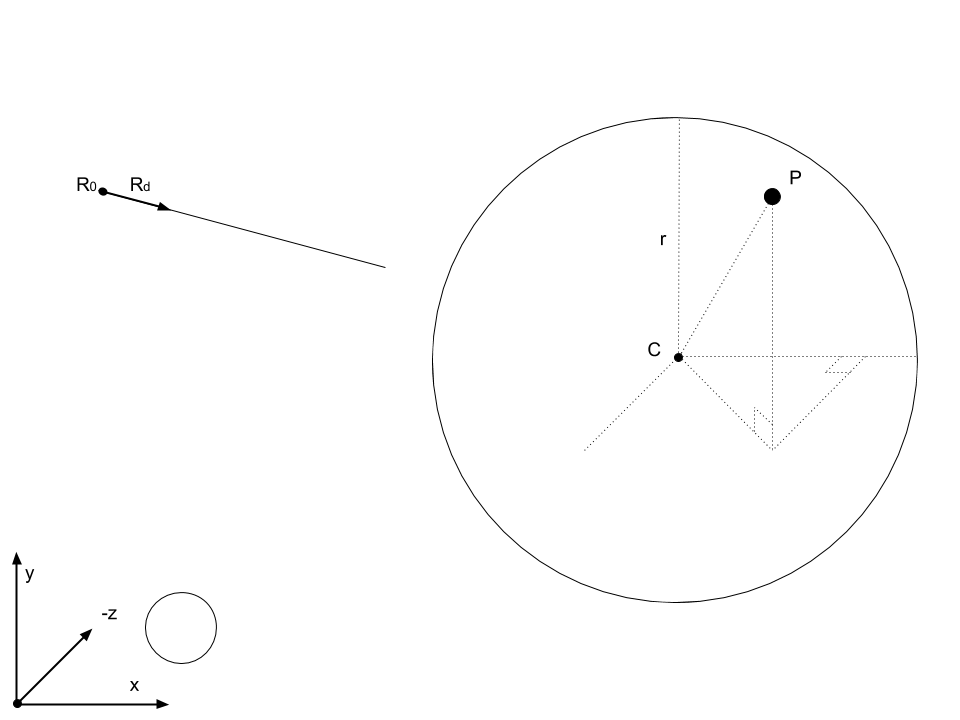
\includegraphics[width=\linewidth]{Figures/ray-sphere-intersection.png}
\decoRule
\caption[ray-sphere-intersection]{Ray-Sphere intersection}
\end{figure}

With known radius and center position, any point on the surface of sphere should match the equation:

\begin{equation}\label{equ:sphere-surface}
(x_{p} - x_{c})^2 + (y_{p} - y_{c})^2 + (z_{p} - z_{c})^2 = r^2
\end{equation}

If the ray intersects with the sphere at any position\emph{P} must match the equation \ref{equ:ray-t} and \ref{equ:sphere-surface}. Therefor the solution of \emph{t} in the cointegrate equation implies whether or not the ray will intersect with the sphere:

\[
\begin{aligned}
(x_{R_{0}} + x_{R_{d}} \cdot t - x_{c})^2 + (y_{R_{0}} + y_{R_{d}} \cdot t - y_{c})^2 + (z_{R_{0}} + z_{R_{d}} \cdot t - z_{c})^2 &= r^2 \\
&\vdots \\
x_{R_{d}}^2 \cdot t^2 + (2 \cdot x_{R_{d}} \cdot (x_{R_{0}} - x_{c})) \cdot t + (x_{R_{0}}^2 - 2 \cdot x_{R_{0}}\cdot x_{c} + x_{c}^2) & \\
+\ y_{R_{d}}^2 \cdot t^2 + (2 \cdot y_{R_{d}} \cdot (y_{R_{0}} - y_{c})) \cdot t + (y_{R_{0}}^2 - 2 \cdot y_{R_{0}}\cdot y_{c} + y_{c}^2) & \\
+\ z_{R_{d}}^2 \cdot t^2 + (2 \cdot z_{R_{d}} \cdot (z_{R_{0}} - z_{c})) \cdot t + (z_{R_{0}}^2 - 2 \cdot z_{R_{0}}\cdot z_{c} + z_{c}^2) &= r^2
\end{aligned}
\]

It can be seen as a quadratic formula:

\begin{equation}\label{equ:sphere-surface-quadratic-formula}
a \cdot t^2 + b \cdot t + c = 0
\end{equation}

At this point, we are able to solved the \emph{t}:

\[
t =
\begin{cases}
\frac{-b \pm \sqrt{b^2 - 4ac}}{2a} & \text{if } b^2 - 4ac > 0 \\
\frac{-b}{2a} & \text{if } b^2 - 4ac = 0 \\
\varnothing & \text{if } b^2 - 4ac < 0
\end{cases}
\]

Then, I take a further step to get rid of formula complexity.

$\because$
\[
\left\{
\begin{array}{lr}
a = x_{R_{d}}^2 + y_{R_{d}}^2 + z_{R_{d}}^2 \\
b = 2 \cdot (x_{R_{d}} \cdot (x_{R_{0}} - x_{c}) + y_{R_{d}} \cdot (y_{R_{0}} - y_{c}) + z_{R_{d}} \cdot (z_{R_{0}} - z_{c})) \\
c = (x_{R_{0}} - x_{c})^2 + (y_{R_{0}} - y_{c})^2 + (z_{R_{0}} - z_{c})^2 - r^2
\end{array}
\right.
\]

$\And$
\[
\left\{
\begin{array}{lr}
\begin{aligned}
\norm{\overrightarrow{R_{d}}} &= \sqrt{x_{R_{d}}^2 + y_{R_{d}}^2 + z_{R_{d}}^2} = 1 \\
\overrightarrow{V_{c\_R_{0}}} &= \overrightarrow{R_{0}} - \overrightarrow{C} = \overrightarrow{(x_{R_{0}} - x_{c}, y_{R_{0}} - y_{c}, z_{R_{0}} - z_{c})}
\end{aligned}
\end{array}
\right.
\]

$\therefore$
\[
\left\{
\begin{array}{lr}
a =1 \\
b = 2 \cdot \overrightarrow{R_{d}} \cdot \overrightarrow{V_{c\_R_{0}}} \\
c = \overrightarrow{V_{c\_R_{0}}} \cdot \overrightarrow{V_{c\_R_{0}}} \cdot r^2
\end{array}
\right.
\]

And the solution for \emph{t} can also be optimized:

$\because$
\[
\begin{array}{lr}
\frac{-b \pm \sqrt{b^2 - 4ac}}{2a} = -(\frac{b}{2a}) \pm \sqrt{(\frac{b}{2a})^2 - \frac{4ac}{4a^2}} = -0.5b \pm \sqrt{(0.5b)^2 - c} \\
B = 0.5b\\
F = B^2 - c
\end{array}
\]

$\therefore$
\[
t =
\begin{cases}
 -B \pm \sqrt{F} & \text{if } F > 0 \\
-B & \text{if } F = 0 \\
\varnothing & \text{if } F < 0
\end{cases}
\]

And the match collision position for each \emph{t} is:

\begin{equation}\label{equ:ray-sphere-intersection}
\overrightarrow{P} = \overrightarrow{R_{0}} + \overrightarrow{R_{d}} \cdot t
\end{equation}


%****************************************************************
\section{Section 2}
asdasd

\subsection{Subsection 1}
asdasdasd

\subsection{Subsection 2}
asdasdasdasd

%****************************************************************
\section{Section 3}

\subsection{Subsection 1}
asdasdasd

\subsection{Subsection 2}
asdasdasdasd

\subsection{Subsection 3}
asdasdasd

%****************************************************************
\section{Section 4}

